\section{Introduction}\label{sec:intro}

The proliferation of Internet of Things (IoT) devices and the increasing complexity of enterprise networks have fundamentally shifted the landscape of cybersecurity. Modern cyberattacks, particularly Advanced Persistent Threats (APTs) and lateral movement strategies, no longer rely on isolated, easily detectable exploits. Instead, they manifest as coordinated sequences of subtle, individually stealthy actions distributed across multiple hosts \cite{Moustafa2015unswnb15}. Traditional Intrusion Detection Systems (IDS), which evaluate network flows or packets in isolation, frequently fail to capture the broader spatial and temporal context necessary to detect these sophisticated campaigns.

To address this limitation, recent research has increasingly turned to Graph Neural Networks (GNNs) for intrusion detection \cite{Lo2022egraphsage, Zhang2026aedgnn}. By representing network entities (such as IP addresses or endpoints) as nodes and communication flows as edges, GNN-based IDSs explicitly model the topological structure of the network. Approaches like E-GraphSAGE \cite{Lo2022egraphsage} and recent multi-granularity frameworks \cite{Liu2025mgfgnn} have demonstrated significant improvements in detecting complex attacks by leveraging message-passing mechanisms to aggregate neighbourhood information. However, the majority of existing GNN-IDS methods formulate the problem as a discrete-time, supervised classification task. This formulation suffers from two critical drawbacks: first, it requires extensive labelled data encompassing all possible attack vectors, leaving the system vulnerable to zero-day exploits; second, it treats network traffic as a sequence of static snapshots, failing to natively capture the continuous, underlying dynamical processes that govern network behaviour over time.

In this paper, we introduce SIREN (Stochastic It\=o Residual on Embedded Networks), a fundamentally novel approach that models a monitored network as a continuous-time dynamical system on a graph. Rather than training a classifier to distinguish between specific attack signatures and benign traffic, SIREN learns the natural, continuous evolution of the network's state. We hypothesise that under normal operation, the network traffic features of interconnected hosts evolve according to a system of graph-coupled It\=o stochastic differential equations (SDEs), eventually converging to a well-defined, unique stationary distribution. 

SIREN leverages score-matching techniques \cite{Song2021sde} to learn the score function (the gradient of the log-probability density) of this normal stationary distribution. At inference time, the system continuously monitors the network state and computes the empirical score of the observed traffic. By measuring the discrepancy between the model-predicted score and the empirical score—a metric we term the \textit{Stein residual}—SIREN can identify when a node's trajectory deviates from expected normal behaviour. Crucially, by aggregating these Stein residuals across the network graph, SIREN amplifies the weak anomaly signals produced by lateral movement attacks, exposing coordinated malicious activities that would remain hidden if hosts were analysed independently.

\begin{figure}[htpb]
    \centering
    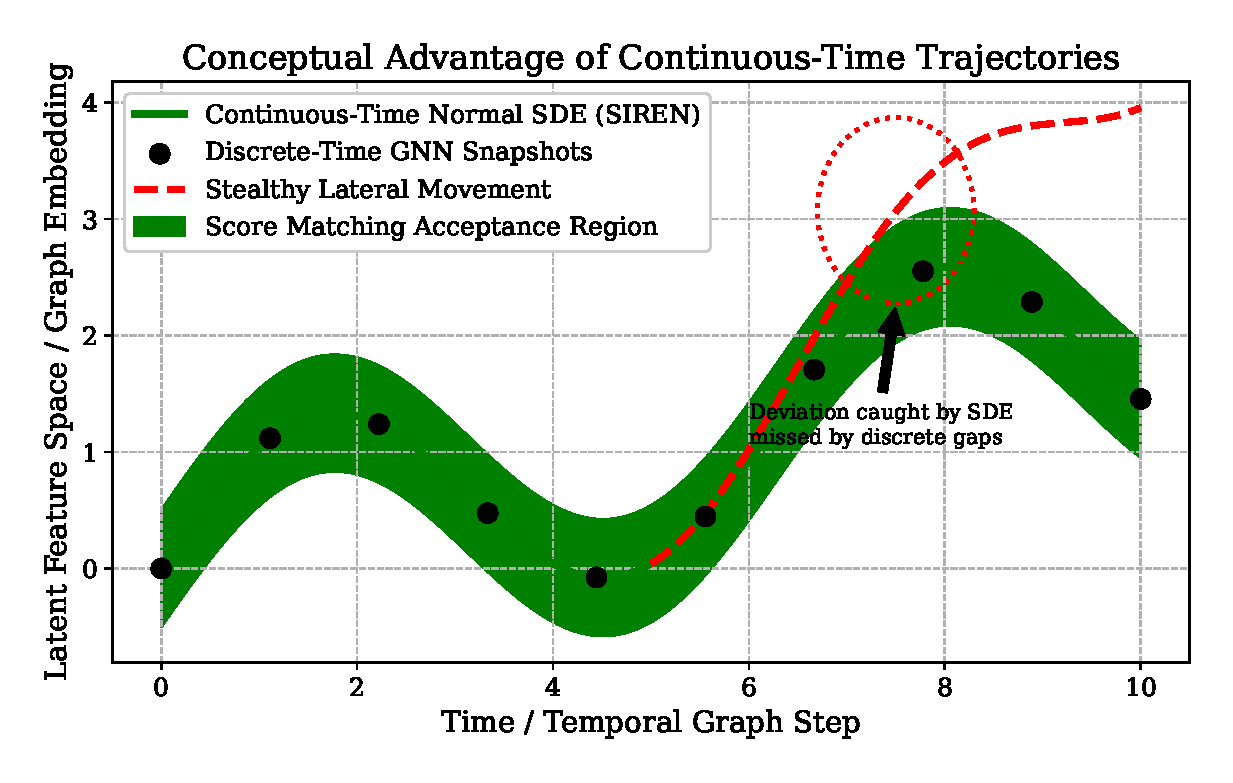
\includegraphics[width=0.8\linewidth]{figures/intro_concept.eps}
    \caption{Conceptual comparison of discrete-time GNN snapshots versus SIREN's continuous-time tracking. Standard graph snapshots leave temporal gaps where stealthy lateral movement can branch off unnoticed. By modeling the normal traffic evolution as a continuous SDE trajectory, SIREN can immediately flag out-of-distribution deviations via score matching.}
    \label{fig:intro_concept}
\end{figure}

As illustrated in Figure \ref{fig:intro_concept}, relying purely on fixed-interval discrete snapshots creates blind spots. An attacker executing lateral movement can carefully pace their actions to fall below the detection threshold at any single discrete timestep. In contrast, SIREN tracks the continuous latent trajectory; even subtle, sub-threshold deviations compound across the continuous SDE formulation, shifting the state out of the high-probability acceptance region and triggering an anomaly alert.

The main contributions of this work are as follows:
\begin{itemize}
    \item We propose a continuous-time formulation of network intrusion detection, modelling host feature trajectories via graph-coupled It\=o SDEs that capture both autonomous node dynamics and topological mean-reversion.
    \item We introduce the \textit{Stein residual} as a mathematically grounded, unsupervised anomaly signal. By evaluating the discrepancy between a learned score network and short-window Kernel Density Estimates (KDE), our approach detects distributional shifts without relying on labelled attack data.
    \item We present a graph-aware aggregation mechanism for Stein residuals, specifically designed to propagate anomaly signals across connected hosts and expose coordinated lateral movement attacks.
    \item We conduct extensive experiments on standard benchmark datasets (UNSW-NB15 and CIC-IDS2018), demonstrating that SIREN outperforms state-of-the-art discrete-time GNN baselines, particularly in terms of False Alarm Rate (FAR) and robustness to feature noise and edge perturbations.
\end{itemize}

The remainder of this paper is structured as follows: Section \ref{sec:related} reviews related work in GNN-based intrusion detection and continuous-time graph models. Section \ref{sec:method} details the SIREN methodology, including graph construction, the SDE formulation, the score network architecture, and the training and inference algorithms. Section \ref{sec:experiments} presents our experimental setup and results, and Section \ref{sec:conclusion} concludes the paper.
